\begin{center}
	\textbf{{\Huge ĐỀ 008: Lê Thánh Tông -- Nguyễn Khuyến HCM tháng 9}}
\end{center}
\subsubsection*{Phần I. Thí sinh trả lời từ câu 1 đến câu 12, mỗi câu hỏi chọn một phương án.}
\setcounter{bt}{0}\setcounter{bt}{0}\setlist[enumerate,1]{label=\quad\bfseries\Alph*.}
\begin{baitap}
	%\textbf{Câu 1.}
	Cho hàm số $y=f(x)$ có đạo hàm trên $\mathbb{R}$ thỏa $f'(x) < 0, \forall x \in (1; 2)$ và $f'(x) > 0, \forall x \in (2; 3)$. Phát biểu nào sau đây là đúng?
	\begin{enumerate}
		\item Hàm số $y=f(x)$ đồng biến trên cả hai khoảng $(1; 2)$ và $(2; 3)$.
		\item Hàm số $y=f(x)$ nghịch biến trên cả hai khoảng $(1; 2)$ và $(2; 3)$.
		\item Hàm số $y=f(x)$ đồng biến trên khoảng $(1; 2)$ và nghịch biến trên khoảng $(2; 3)$.
		\item Hàm số $y=f(x)$ nghịch biến trên khoảng $(1; 2)$ và đồng biến trên khoảng $(2; 3)$.
	\end{enumerate}
	\begin{traloi}
		\dapan{D}
		Vì $f'(x) < 0, \forall x \in (1; 2)$ nên hàm số nghịch biến trên khoảng $(1; 2)$.
		Vì $f'(x) > 0, \forall x \in (2; 3)$ nên hàm số đồng biến trên khoảng $(2; 3)$.
	\end{traloi}
\end{baitap}

\begin{baitap}
	%\textbf{Câu 2.}
	Giá trị cực đại của hàm số $f(x) = 2x^3 - 9x^2 - 24x + 11$ là
	\begin{multicols}{4}
		\begin{enumerate}
			\item $-1$.
			\item $24$.
			\item $4$.
			\item $-111$.
		\end{enumerate}
	\end{multicols}
	\begin{traloi}
		\dapan{B}
		Ta có $f'(x) = 6x^2 - 18x - 24 = 6(x^2 - 3x - 4)$.
		$f'(x) = 0 \Leftrightarrow \left[
		\begin{array}{l}
				 x = -1\\
				x = 4
		\end{array}
		\right.$
		Đạo hàm đổi dấu từ dương sang âm qua $x = -1$, do đó $x = -1$ là điểm cực đại.
		Giá trị cực đại của hàm số là $f(-1)  = 24$.
	\end{traloi}
\end{baitap}

\begin{baitap}
	%\textbf{Câu 3.}
	Cho lăng trụ $ABC.A'B'C'$. Khẳng định nào sau đây đúng?
	\begin{multicols}{4}
		\begin{enumerate}
			\item $\overrightarrow{BA} + \overrightarrow{A'C'} = \overrightarrow{BC}$.
			\item $\overrightarrow{BA} + \overrightarrow{A'C'} = \overrightarrow{BC'}$.
			\item $\overrightarrow{BA} + \overrightarrow{A'C'} = \overrightarrow{C'B}$.
			\item $\overrightarrow{BA} + \overrightarrow{A'C'} = \overrightarrow{B'C'}$.
		\end{enumerate}
	\end{multicols}
	\begin{traloi}
		\dapan{A}
		Vì $ABC.A'B'C'$ là hình lăng trụ nên $\overrightarrow{A'C'} = \overrightarrow{AC}$.
		Do đó, $\overrightarrow{BA} + \overrightarrow{A'C'} = \overrightarrow{BA} + \overrightarrow{AC} = \overrightarrow{BC}$.
	\end{traloi}
\end{baitap}

\begin{baitap}
	%\textbf{Câu 4.}
	Hàm số $y=f(x)$ xác định trên đoạn $[-1; 6]$ và có đồ thị như hình vẽ. 
	\begin{center}
		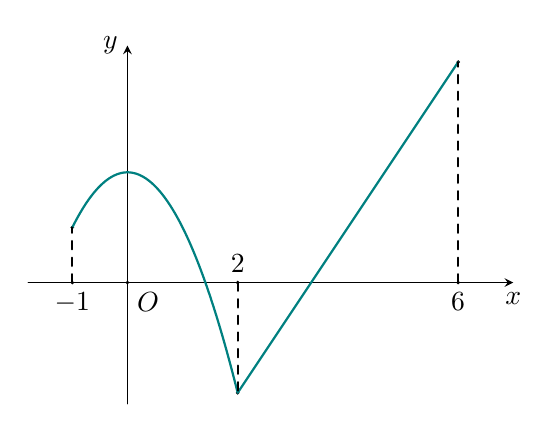
\begin{tikzpicture}[>=stealth, line cap=round, line join=round, scale=.7]
			
			% Trục tọa độ
			\draw[->] (-1.8,0) -- (7,0) node[below] {$x$};
			\draw[->] (0,-2.2) -- (0,4.3) node[left] {$y$};
			
			% Các điểm trên trục Ox
			\fill (-1,0) circle (1pt);
			\fill (0,0) circle (1pt);
			\fill (2,0) circle (1pt);
			\fill (6,0) circle (1pt);
			\fill (2,-2) circle (1pt);
			\fill (-1,1) circle (1pt);
			\fill (6,4) circle (1pt);
			
			% Nhãn
			\node[below] at (-1,0) {$-1$};
			\node[below right] at (0,0) {$O$};
			\node[above] at (2,0) {$2$};
			\node[below] at (6,0) {$6$};
			
			% Parabol: đi qua (-1,1), đạt cực đại tại (0,2), đi qua (2,-2)
			\draw[teal, thick, domain=-1:2, samples=100]
			plot (\x,{2-\x*\x});
			
			% Đoạn thẳng từ (2,-2) đến (6,4)
			\draw[teal, thick]
			(2,-2) -- (6,4);
			
			% Các đường gióng nét đứt
			\draw[dashed, thick] (-1,0) -- (-1,1);
			\draw[dashed, thick] (2,0) -- (2,-2);
			\draw[dashed, thick] (6,0) -- (6,4);
			
		\end{tikzpicture}
	\end{center}
	Hàm số đã cho nghịch biến trên khoảng nào sau đây?
	\begin{multicols}{4}
		\begin{enumerate}
			\item $(-1; 2)$.
			\item $(0; 2)$.
			\item $(2; 6)$.
			\item $(-2; 0)$.
		\end{enumerate}
	\end{multicols}
	\begin{traloi}
		\dapan{B}
		Dựa vào đồ thị, trên khoảng $(0; 2)$ đồ thị đi xuống từ trái sang phải, suy ra hàm số nghịch biến trên khoảng $(0; 2)$.
	\end{traloi}
\end{baitap}

\begin{baitap}
	%\textbf{Câu 5.}
	Cho tứ diện $ABCD$. Lấy $G$ là trọng tâm của tam giác $ABC$. Phát biểu nào sau đây là \textbf{sai}?
	\begin{multicols}{2}
		\begin{enumerate}
			\item $\overrightarrow{GA} + \overrightarrow{GB} + \overrightarrow{GC} = \overrightarrow{0}$.
			\item $\overrightarrow{GA} + \overrightarrow{GB} + \overrightarrow{GC} + \overrightarrow{GD} = \overrightarrow{0}$.
			\item $\overrightarrow{GD} - \overrightarrow{GA} = \overrightarrow{AD}$.
			\item $\overrightarrow{DA} + \overrightarrow{DB} + \overrightarrow{DC} = 3\overrightarrow{DG}$.
		\end{enumerate}
	\end{multicols}
	\begin{traloi}
		\dapan{B}
		Vì $G$ là trọng tâm của tam giác $ABC$ nên $\overrightarrow{GA} + \overrightarrow{GB} + \overrightarrow{GC} = \overrightarrow{0}$ là khẳng định đúng.
		Do đó $\overrightarrow{GA} + \overrightarrow{GB} + \overrightarrow{GC} + \overrightarrow{GD} = \overrightarrow{0} + \overrightarrow{GD} = \overrightarrow{GD} \ne \overrightarrow{0}$ (vì $D$ không trùng $G$).
		Vậy phát biểu B là sai.
	\end{traloi}
\end{baitap}

\begin{baitap}
	%\textbf{Câu 6.}
	Một chiếc hộp hình lập phương $ABCD.A'B'C'D'$ có cạnh bằng \qty{12}{\centi\meter}, mặt trên $A'B'C'D'$ không nắp. Có một con kiến ở đỉnh $A$ bên ngoài hộp và một miếng mồi của kiến tại điểm $O$ là tâm đáy $ABCD$ ở bên trong hộp. Quãng đường ngắn nhất mà con kiến tìm đến miếng mồi (\textit{làm tròn đến hai chữ số thập phân}) là
	\begin{multicols}{4}
		\begin{enumerate}
			\item \qty{32{,}49}{\centi\meter}.
			\item \qty{36{,}29}{\centi\meter}.
			\item \qty{12}{\centi\meter}.
			\item \qty{30{,}59}{\centi\meter}.
		\end{enumerate}
	\end{multicols}
	\begin{traloi}
		\dapan{D}
		Con kiến ở \(A\) phía ngoài hộp, còn \(O\) nằm ở mặt đáy phía trong hộp. Vì vậy để đến \(O\), kiến phải đi qua ba mặt: mặt bên phía ngoài \(\to\) mặt bên phía trong \(\to\) mặt đáy.  Do tính đối xứng, ta chọn mặt bên \(ABB'A'\) và trải phẳng ba mặt mà kiến đi qua như hình sau:
			\begin{center}
				\begin{tikzpicture}[
					line cap=round,
					line join=round,
					>=stealth,
					scale=0.25
					]
					% Các điểm trên hình trải phẳng
					\coordinate (A)  at (0,0);
					\coordinate (B)  at (12,0);
					
					% Mặt ngoài
					\coordinate (A1) at (0,12);
					\coordinate (B1) at (12,12);
					
					
					\coordinate (M) at (8,12);
					\coordinate (N) at (3,24);
					
					% Mặt trong sau khi trải
					\coordinate (A2) at (0,24);
					\coordinate (B2) at (12,24);
					
					% Phần đáy đến tâm O
					\coordinate (O)  at (6,30);
					\coordinate (D2) at (0,30);
					\coordinate (C2) at (12,30);
					
					% Hai hình vuông biểu diễn mặt ngoài và mặt trong
					\draw[thick] (A) rectangle (B1);
					\draw[thick] (A1) rectangle (B2);
					
					% Nửa đáy chứa tâm O
					\draw[thick] (A2) -- (D2) -- (C2) -- (B2);
					
					% Đường đi ngắn nhất
					\draw[very thick] (A) -- (O);
					\draw[red, very thick] (A) -- (M) -- (N) -- (O);
					
					
					\fill (A) circle (5pt);
					\fill (M) circle (5pt);
					\fill (N) circle (5pt);
					\fill (O) circle (5pt);
					
					% Nhãn điểm
					\node[below left] at (A) {$A$};
					\node[left] at (A1) {$A'$};
					\node[left] at (A2) {$A$};
					\node[above right] at (O) {$O$};
					\node[below right] at (B) {$B$};
					\node[right] at (B1) {$B'$};
					\node[right] at (B2) {$B$};
					
					\node[below right] at (M) {$M$};
					\node[above left] at (N) {$N$};
					
					% Chú thích các mặt
					\node[rotate=90] at (-2.5,6)
					{\small Mặt ngoài};
					
					\node[rotate=90] at (-2.5,18)
					{\small Mặt trong};
					
					\node at (7,27)
					{\small Đáy};
					
					% Kích thước 12 + 12 + 6
					\draw[<->] (-5,0) -- (-5,12)
					node[midway,left] {$12$};
					
					\draw[<->] (-5,12) -- (-5,24)
					node[midway,left] {$12$};
					
					\draw[<->] (-5,24) -- (-5,30)
					node[midway,left] {$6$};
					
					% Kích thước ngang 6
					\draw[dashed] (O) -- (0,30);
					\draw[<->] (0,32) -- (6,32)
					node[midway,above] {$6$};
					
					% Chú thích đường ngắn nhất
					\node[
					rotate=78.7,
					fill=white,
					inner sep=2pt
					] at (3,15)
					{\small Đường đi ngắn nhất};
					
				\end{tikzpicture}
			\end{center}		
		\begin{itemize}
			\item Đầu tiên, kiến bò trên mặt ngoài \(ABB'A'\) từ điểm \(A\) đến điểm $ M $ nào đó nằm trên mép trên \(A'B'\);
			\item Sau khi đến mép \(A'B'\), kiến bò trên mặt trong của chính mặt bên \(ABB'A'\) đó từ điểm \(M\) đến điểm $ N $ nào đó trên cạnh \(AB\);
			\item Trên mặt đáy \(ABCD\), kiến bò từ điểm $ N $  tới điểm \(O\) là tâm hình vuông \(ABCD\).
		\end{itemize}
		Rõ ràng, tổng quãng đường kiến bò được là $ AM+MN+NO $ mà ta luôn có
		$$ AM+MN+NO  \geqslant AO. $$
		Do đó, đường đi ngắn nhất của kiến có độ dài là
		\[
		\sqrt{30^2+6^2}
		\approx30{,}59\text{ cm}.
		\]
		
		Vậy quãng đường ngắn nhất con kiến phải đi là \(30{,}59\) cm.
	\end{traloi}
\end{baitap}

\begin{baitap}
	%\textbf{Câu 7.}
	Giá trị nhỏ nhất của hàm số $f(x)=x^4-8x^2+a$, ($a\in\mathbb{R}$) trên đoạn $[-1; 3]$ bằng
	\begin{multicols}{4}
		\begin{enumerate}
			\item $-6$.
			\item $a$.
			\item $-16+a$.
			\item $9+a$.
		\end{enumerate}
	\end{multicols}
	\begin{traloi}
		\dapan{C}
		Ta có $f'(x)=4x^3-16x=4x(x^2-4)=0 \Leftrightarrow x=0 \in [-1; 3]$ hoặc $x=2 \in [-1; 3]$ hoặc $x=-2 \notin [-1; 3]$.
		Tính các giá trị: $f(-1)=a-7$, $f(0)=a$, $f(2)=a-16$, $f(3)=a+9$.
		So sánh các giá trị, ta được $\min\limits_{[-1; 3]} f(x) = f(2) = -16+a$.
	\end{traloi}
\end{baitap}

\begin{baitap}
	%\textbf{Câu 8.}
	Hàm số $y=f(x)$ xác định trên đoạn $[-1; 5]$ và có đồ thị như hình vẽ. 
	\begin{center}
		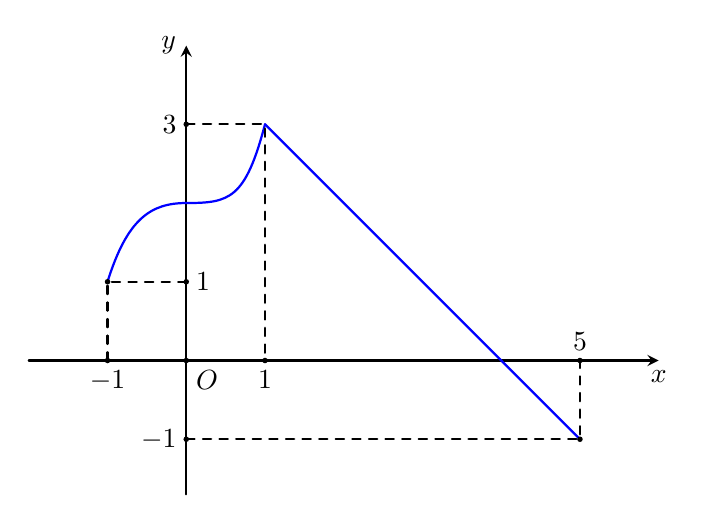
\begin{tikzpicture}[>=stealth, line cap=round, line join=round, scale=1]
			
			% Trục tọa độ
			\draw[->, thick] (-2,0) -- (6,0) node[below] {$x$};
			\draw[->, thick] (0,-1.7) -- (0,4) node[left] {$y$};
			
			% Đường cong trên [-1,1]
			\draw[blue, thick]
			(-1,1)
			.. controls (-0.75,1.8) and (-0.45,2) .. (0,2)
			.. controls (0.55,2) and (0.75,2.05) .. (1,3);
			
			% Đoạn thẳng từ (1,3) đến (5,-1)
			\draw[blue, thick] (1,3) -- (5,-1);
			
			% Các đường gióng nét đứt
			\draw[dashed, thick] (-1,0) -- (-1,1) -- (0,1);
			\draw[dashed, thick] (0,3) -- (1,3) -- (1,0);
			\draw[dashed, thick] (0,-1) -- (5,-1) -- (5,0);
			
			% Các điểm - bán kính 1pt
			\fill (-1,0) circle (1pt);
			\fill (-1,1) circle (1pt);
			
			\fill (0,-1) circle (1pt);
			\fill (0,0) circle (1pt);
			\fill (0,1) circle (1pt);
			\fill (0,3) circle (1pt);
			
			\fill (1,0) circle (1pt);
			
			\fill (5,0) circle (1pt);
			\fill (5,-1) circle (1pt);
			
			% Nhãn trên trục Ox
			\node[below] at (-1,0) {$-1$};
			\node[below right] at (0,0) {$O$};
			\node[below] at (1,0) {$1$};
			\node[above] at (5,0) {$5$};
			
			% Nhãn trên trục Oy
			\node[left] at (0,-1) {$-1$};
			\node[right] at (0,1) {$1$};
			\node[left] at (0,3) {$3$};
			
		\end{tikzpicture}
	\end{center}
	Tập giá trị của hàm số $y=f(x)$ trên đoạn $[-1; 5]$ là
	\begin{multicols}{4}
		\begin{enumerate}
			\item $[-1; 5]$.
			\item $[1; 3]$.
			\item $[-1; 3]$.
			\item $[1; 5]$.
		\end{enumerate}
	\end{multicols}
	\begin{traloi}
		\dapan{C}
		Quan sát đồ thị hàm số trên đoạn $[-1; 5]$, ta thấy giá trị nhỏ nhất của $y$ là $-1$ (tại $x=5$) và giá trị lớn nhất của $y$ là $3$ (tại $x=1$).
		Do đó, tập giá trị của hàm số $y=f(x)$ là $[-1; 3]$.
	\end{traloi}
\end{baitap}
\begin{baitap}
	%\textbf{Câu 9.}
	Mỗi ngày bác Bình đều đi bộ để rèn luyện sức khoẻ. Quãng đường đi bộ mỗi ngày (đơn vị: $\mathrm{km}$) của bác Bình trong $20$ ngày được thống kê lại ở bảng sau:
	\begin{center}
		\begin{tabular}{|c|c|c|c|c|c|}
			\hline
			\textbf{Quãng đường} & $[2{,}7; 3{,}0)$ & $[3{,}0; 3{,}3)$ & $[3{,}3; 3{,}6)$ & $[3{,}6; 3{,}9)$ & $[3{,}9; 4{,}2)$ \\
			\hline
			\textbf{Số ngày} & $3$ & $6$ & $5$ & $4$ & $2$ \\
			\hline
		\end{tabular}
	\end{center}
	Khoảng biến thiên của mẫu số liệu ghép nhóm trên bằng
	\begin{multicols}{4}
		\begin{enumerate}
			\item $1{,}2$.
			\item $0{,}362$.
			\item $3{,}39$.
			\item $1{,}5$.
		\end{enumerate}
	\end{multicols}
	\begin{traloi}
		\dapan{D}
		Khoảng biến thiên của mẫu số liệu ghép nhóm là $R = 4{,}2 - 2{,}7 = 1{,}5$.
	\end{traloi}
	\end{baitap}		
\begin{baitap}
	%\textbf{Câu 10.}
	Trong không gian $Oxyz$, cho hai điểm $A(1; 1; 2)$ và $B(3; 1; 0)$. Trung điểm của đoạn thẳng $AB$ có tọa độ là
	\begin{multicols}{4}
		\begin{enumerate}
			\item $(2; 1; 1)$.
			\item $(4; 2; 2)$.
			\item $(2; 0; -2)$.
			\item $(1; 0; -1)$.
		\end{enumerate}
	\end{multicols}
	\begin{traloi}
		\dapan{A}
		Tọa độ trung điểm $I$ của $AB$ là $I\left(\frac{1+3}{2}; \frac{1+1}{2}; \frac{2+0}{2}\right) = (2; 1; 1)$.
	\end{traloi}
\end{baitap}

\begin{baitap}
	%\textbf{Câu 11.}
	Đường tiệm cận xiên của đồ thị hàm số $y = \frac{x^2 + 2x - 2}{x - 2}$ là
	\begin{multicols}{4}
		\begin{enumerate}
			\item $y = -x + 3$.
			\item $y = x + 3$.
			\item $y = x - 3$.
			\item $y = x + 4$.
		\end{enumerate}
	\end{multicols}
	\begin{traloi}
		\dapan{D}
		Ta có $y = \frac{x^2 + 2x - 2}{x - 2} = x + 4 + \frac{6}{x - 2}$.
		Do $\lim\limits_{x \to \infty} \frac{6}{x - 2} = 0$ nên đường tiệm cận xiên của đồ thị hàm số là $y = x + 4$.
	\end{traloi}
\end{baitap}

\begin{baitap}
	%\textbf{Câu 12.}
	Trong không gian $Oxyz$, cho điểm $A(-3; 1; -4)$, $B(1; -5; 2)$. Đường thẳng $AB$ cắt mặt phẳng $(Oxy)$ tại điểm
	\begin{multicols}{4}
		\begin{enumerate}
			\item $M\left(-\frac{1}{3}; -3; 0\right)$.
			\item $N\left(\frac{1}{3}; 3; 0\right)$.
			\item $P(0; 3; 1)$.
			\item $Q(-3; 1; 0)$.
		\end{enumerate}
	\end{multicols}
	\begin{traloi}
		\dapan{A}
		Vectơ chỉ phương $\overrightarrow{AB} = (4; -6; 6)$.
		Phương trình tham số của đường thẳng $AB$:
		\[
		\begin{cases}
			x = -3 + 4t \\
			y = 1 - 6t \\
			z = -4 + 6t
		\end{cases}
		\]
		Đường thẳng $AB$ cắt $(Oxy)$ ($z = 0$) tại điểm có $-4 + 6t = 0 \Rightarrow t = \frac{2}{3}$.
		Tọa độ giao điểm là $x = -3 + 4\cdot\frac{2}{3} = -\frac{1}{3}$, $y = 1 - 6\cdot\frac{2}{3} = -3$, $z = 0$, tức điểm $M\left(-\frac{1}{3}; -3; 0\right)$.
	\end{traloi}
\end{baitap}
\subsubsection*{Phần II. Thí sinh trả lời từ câu 1 đến câu 4, trong ý a), b), c), d) ở mỗi câu câu, thí sinh chọn ĐÚNG hoặc SAI.}
\setcounter{bt}{0}\setcounter{bt}{0}\setlist[enumerate,1]{label=\quad\bfseries\alph*)}
\begin{baitap}
	%\textbf{Câu 1.}
	Hàm số $y = f(x)$ liên tục trên $\mathbb{R}$ và có bảng biến thiên như sau:
	\begin{center}
		
\begin{tikzpicture}
			\tkzTabInit[lgt=1.5,espcl=2.5]{$x$ /1, $y'$ /1, $y$ /2}{$-\infty$, $-1$, $1$, $+\infty$}
			\tkzTabLine{,-,0,+,0,-,}
			\tkzTabVar{+/$142$, -/$8$, +/$38$, -/$14$}
		\end{tikzpicture}
	\end{center}
	\begin{enumerate}
		\item Đồ thị hàm số đã cho có hai đường tiệm cận ngang.
		\item Giá trị nhỏ nhất của hàm số trên $(-\infty; +\infty)$ bằng $8$.
		\item Hàm số đồng biến trên $(8; 38)$.
		\item Giá trị lớn nhất của hàm số trên $\mathbb{R}$ bằng $142$.
	\end{enumerate}
	\begin{traloi}
		\dapan{Đúng -- Đúng -- Sai -- Sai}
		
		\begin{enumerate}
			\item \textbf{Đúng}. Ta có \(\lim\limits_{x\to-\infty}f(x)=142\) và \(\lim\limits_{x\to+\infty}f(x)=14\), nên đồ thị có hai tiệm cận ngang \(y=142\) và \(y=14\).
			
			\item \textbf{Đúng}. Từ bảng biến thiên, \(f(-1)=8\) và mọi giá trị khác của hàm số đều lớn hơn hoặc bằng \(8\). Vậy giá trị nhỏ nhất là \(8\).
			
			\item \textbf{Sai}. Khoảng đồng biến phải là khoảng của biến \(x\). Từ bảng biến thiên, hàm số đồng biến trên \((-1;1)\), không phải \((8;38)\).
			
			\item \textbf{Sai}. Ta có \(\lim\limits_{x\to-\infty}f(x)=142\), nhưng hàm số giảm từ \(142\) xuống \(8\) trên \((-\infty;-1)\), nên \(f(x)<142\) với mọi \(x\in\mathbb R\). Do đó hàm số không có giá trị lớn nhất trên \(\mathbb R\).
		\end{enumerate}
	\end{traloi}
\end{baitap}

\begin{baitap}
	%\textbf{Câu 2.}
	Xét tam giác $ABC$ có $AC = 2AB$ và $BC = \qty{10}{\centi\meter}$. Trên cạnh $AC$ lấy điểm $D$ sao cho $AD = \frac{1}{4}AC$, trên cạnh $AB$ lấy điểm $E$ sao cho $AE = \frac{1}{4}AB$, trên cạnh $AD$ lấy điểm $F$ sao cho $AF = \frac{1}{4}AD$ và tiếp tục lấy các điểm $G, H, I, J...$ (vô hạn lần) theo quy luật đó. Xét tính đúng sai các mệnh đề sau.
	\begin{center}
		%!<\usetikzlibrary{calc}>
		
		\begin{tikzpicture}[line cap=round, line join=round, >=stealth, scale=0.95]
			% Define main coordinates for triangle ABC
			% A is top vertex, B is to the left, C is to the bottom right
			\coordinate (A) at (1.0, 3.8);
			\coordinate (B) at (-0.6, 0.7);
			\coordinate (C) at (3.0, -1.5);
			
			% D on AC such that AD = 1/4 AC
			\coordinate (D) at ($(A)!0.25!(C)$);
			
			% E on AB such that AE = 1/4 AB
			\coordinate (E) at ($(A)!0.25!(B)$);
			
			% F on AD such that AF = 1/4 AD
			\coordinate (F) at ($(A)!0.25!(D)$);
			
			% Draw main triangle sides
			\draw[thick] (A) -- (B) -- (C) -- cycle;
			
			% Draw construction segments: BD, DE, EF
			\draw[thick] (B) -- (D);
			\draw[thick] (D) -- (E);
			\draw[thick] (E) -- (F);
			
			% Plot points
			\foreach \p in {A, B, C, D, E, F} {
				\fill (\p) circle (1.8pt);
			}
			
			% Vertex labels matching the given image layout
			\node[above, font=\small] at (A) {$A$};
			\node[left, font=\small] at (B) {$B$};
			\node[right, font=\small] at (C) {$C$};
			\node[right, font=\small] at (D) {$D$};
			\node[left, font=\small] at (E) {$E$};
			\node[right, font=\small] at (F) {$F$};
		\end{tikzpicture}
	\end{center}
	\begin{enumerate}
		\item $\frac{AB}{AC} = \frac{AD}{AB}$.
		\item Tam giác $ABD$ đồng dạng với tam giác $ABC$.
		\item $BD = \qty{5}{\centi\meter}$; $DE = \qty{3}{\centi\meter}$.
		\item Độ dài đường gấp khúc $CBDEFGH\ldots$ bằng \qty{20}{\centi\meter}.
	\end{enumerate}
	\begin{traloi}
		\dapan{Đúng -- Sai -- Sai -- Đúng}
		
		\begin{enumerate}
			\item \textbf{Đúng}. Vì $AC = 2AB \Rightarrow \frac{AB}{AC} = \frac{1}{2}$. Lại có $AD = \frac{1}{4}AC = \frac{1}{2}AB \Rightarrow \frac{AD}{AB} = \frac{1}{2}$. Vậy $\frac{AB}{AC} = \frac{AD}{AB}$.
			\item \textbf{Sai}. Xét $\triangle ABD$ và $\triangle ACB$ có $\widehat{A}$ chung và $\frac{AB}{AC} = \frac{AD}{AB} = \frac{1}{2}$, nên $\triangle ABD \sim \triangle ACB$, chứ không phải $ \triangle ABC. $
			\item \textbf{Sai}. Vì $\triangle ABD \sim \triangle ACB$ tỉ số $k = \frac{1}{2}$ nên $BD = \frac{1}{2}BC = \qty{5}{\centi\meter}$. Tương tự, $\triangle ADE \sim \triangle ABD$ tỉ số $\frac{1}{4}$ nên $DE = \frac{1}{4}BD = \qty{1{,}25}{\centi\meter} \neq \qty{3}{\centi\meter}$.
			\item \textbf{Đúng}. Độ dài các đoạn nối tiếp nhau tạo thành một cấp số nhân lùi vô hạn với $u_1 = BC = 10$ và công bội $q = \frac{1}{2}$, nên tổng độ dài $S = \frac{10}{1 - \frac{1}{2}} = \qty{20}{\centi\meter}$.
		\end{enumerate}
	\end{traloi}
\end{baitap}
\begin{baitap}
	%\textbf{Câu 3.}
	Hình vẽ sau, điểm $ M $ mô tả vị trí của máy bay vào thời điểm $9\mathrm{h}30$ phút. Biết các đơn vị trên hình tính theo đơn vị $\mathrm{km}$. Trong các khẳng định sau đây, khẳng định nào đúng, khẳng định nào sai?
	\begin{center}
		%!<\usetikzlibrary{shapes.symbols, calc}>
		
		\begin{tikzpicture}[line cap=round, line join=round, >=stealth, scale=1.1]
			
			% 3D projection axes setup (cavalier-like projection matching the figure)
			% x points bottom-left, y points right, z points up
			\coordinate (O) at (0, 0);
			\coordinate (X) at (-1.8, -1.8);
			\coordinate (Y) at (4.0, 0);
			\coordinate (Z) at (0, 4.0);
			
			% Coordinates on the axes
			\coordinate (Px) at (-1.2, -1.2); % Position for 150 on x-axis
			\coordinate (Py) at (2.4, 0);     % Position for 300 on y-axis
			\coordinate (Pz) at (0, 3.0);     % Position for 9 on z-axis
			
			% Coordinates in space
			\coordinate (Pxy) at ($(Px) + (Py)$); % Projection on xy plane
			\coordinate (Airplane) at ($(Pxy) + (Pz)$); % Airplane position (150, 300, 9)
			
			% Dashed projection lines
			\draw[dashed, thick] (Px) -- (Pxy);
			\draw[dashed, thick] (Py) -- (Pxy);
			\draw[dashed, thick] (O) -- (Pxy);
			\draw[dashed, thick] (Pxy) -- (Airplane);
			\draw[dashed, thick] (Pz) -- (Airplane);
			
			% Coordinate axes
			\draw[->, thick] (O) -- (X) node[left] {$x$} node[right=2pt, font=\small] {(Nam)};
			\draw[->, thick] (O) -- (Y) node[above] {$y$} node[below=2pt, font=\small] {(Đông)};
			\draw[->, thick] (O) -- (Z) node[left] {$z$};
			
			% Origin
			\node[above left, font=\small] at (O) {$O$};
			
			% Mark values on axes with small dots
			\fill (Px) circle (1pt) node[left=2pt, font=\small] {$150$};
			\fill (Py) circle (1pt) node[above=2pt, font=\small] {$300$};
			\fill (Pz) circle (1pt) node[left=2pt, font=\small] {$9$};
			
			% Mark values on axes
			\fill (Px) circle (1pt)
			node[left=2pt, font=\small] {$150$};
			
			\fill (Py) circle (1pt)
			node[above=2pt, font=\small] {$300$};
			
			\fill (Pz) circle (1pt)
			node[left=2pt, font=\small] {$9$};
			
			% % Right-angle markers
			% \tkzMarkRightAngle[size=0.3, thick](O,Px,Pxy)
			% \tkzMarkRightAngle[size=0.3, thick](O,Py,Pxy)
			% \tkzMarkRightAngle[size=0.3,thick](O,Pz,Airplane)
			
			% Airplane
			\fill (Airplane) circle (1.5pt);
			\node[font=\large, right] at (Airplane) {$ M $};
			
%			% Airplane symbol at position
%			\fill (Airplane) circle (1.5pt);
%			\node[rotate=20, font=\large] at (Airplane) {$ M $};
			
		\end{tikzpicture}
	\end{center}
	\begin{enumerate}
		\item Máy bay đang ở độ cao \qty{9}{\kilo\meter}.
		\item Tọa độ của máy bay $(300; 150; 9)$.
		\item Phi công để máy bay ở chế độ tự động với vận tốc theo hướng đông là \qty{750}{\kilo\meter\per\hour}, độ cao không đổi. Biết rằng gió thổi theo hướng đông với vận tốc \qty{10}{\meter\per\second}. Giả sử vận tốc và hướng gió không đổi thì lúc $10\mathrm{h}30$ phút máy bay ở tọa độ $(150; 1086; 9)$.
		\item Sau khi bay đến vị trí lúc $10\mathrm{h}30$ thì máy bay bay theo hướng ngược lại với vận tốc \qty{800}{\kilo\meter\per\hour} với độ cao không đổi, biết lúc đó trời lặng gió thì lúc $11\mathrm{h}$ máy bay ở tọa độ $(686; 150; 9)$.
	\end{enumerate}
	\begin{traloi}
				\dapan{Đúng -- Sai -- Đúng -- Sai}
		\begin{enumerate}
			\item \textbf{Đúng}. Độ cao của máy bay chính là cao độ $z = \qty{9}{\kilo\meter}$.
			\item \textbf{Sai}. Dựa vào hệ trục tọa độ $Oxyz$, hoành độ $x = 150$, tung độ $y = 300$, cao độ $z = 9$. Do đó tọa độ của máy bay là $(150; 300; 9)$.
			\item \textbf{Đúng}. Đổi \qty{10}{\meter\per\second} = \qty{36}{\kilo\meter\per\hour}. Vận tốc tổng cộng theo hướng đông (trục $Oy$) là $750 + 36 = \qty{786}{\kilo\meter\per\hour}$.
			Thời gian bay từ $9\mathrm{h}30$ đến $10\mathrm{h}30$ là $1$ giờ.
			Tung độ mới $y = 300 + 786 \cdot 1 = 1086$. Tọa độ mới là $(150; 1086; 9)$.
			\item \textbf{Sai}. Máy bay bay theo hướng ngược lại (hướng tây, ngược chiều dương của trục $Oy$) với vận tốc \qty{800}{\kilo\meter\per\hour} trong $0{,}5$ giờ.
			Quãng đường đi được là $800 \cdot 0{,}5 = \qty{400}{\kilo\meter}$.
			Tung độ mới $y = 1086 - 400 = 686$. Do đó tọa độ mới phải là $(150; 686; 9)$.
		\end{enumerate}
	\end{traloi}
\end{baitap}
\begin{baitap}
	%\textbf{Câu 4.}
	Khảo sát chiều cao của 20 học sinh nam lớp 12A của một trường THPT X, người ta được kết quả thống kê trong bảng sau:
	\begin{center}
		\begin{tabular}{|c|c|c|c|c|c|}
			\hline
			\textbf{Chiều cao ($\mathrm{cm}$)} & $[160; 165)$ & $[165; 170)$ & $[170; 175)$ & $[175; 180)$ & $[180; 185)$ \\
			\hline
			\textbf{Số học sinh} & 3 & 5 & 7 & 4 & 1 \\
			\hline
		\end{tabular}
	\end{center}
	\begin{enumerate}
		\item Gọi $x_1; x_2; \ldots; x_{20}$ là mẫu số liệu gốc gồm chiều cao của 20 học sinh trên được xếp theo thứ tự không giảm. Khi đó, $x_3 \in [165; 170)$ và $x_9 \in [170; 175)$.
		\item Tứ phân vị thứ ba của mẫu số liệu ghép nhóm đã cho bằng 175.
		\item Khoảng tứ phân vị của mẫu số liệu ghép nhóm đã cho là $\Delta Q = Q_3 - Q_1 = 8{,}5$.
		\item Chọn ngẫu nhiên một học sinh trong nhóm khảo sát nói trên, xác suất chọn được học sinh có chiều cao từ \qty{175}{\centi\meter} trở lên bằng $0{,}25$.
	\end{enumerate}
	\begin{traloi}
		\dapan{Sai -- Đúng -- Sai -- Đúng}
		
		\begin{enumerate}
			\item \textbf{Sai}. Ba học sinh đầu tiên thuộc nhóm \([160;165)\), nên \(x_3\in[160;165)\). Do \(3+5=8\), nên \(x_9\in[170;175)\).
			
			\item \textbf{Đúng}. Vị trí \(Q_3\) là \(\frac{3n}{4}=15\). Nhóm chứa \(Q_3\) là \([170;175)\), nên \(Q_3=170+\frac{15-8}{7}\cdot5=175\).
			
			\item \textbf{Sai}. \(Q_1\) thuộc nhóm \([165;170)\), nên \(Q_1=165+\frac{5-3}{5}\cdot5=167\). Do đó \(\Delta Q=175-167=8\).
			
			\item \textbf{Đúng}. Có \(4+1=5\) học sinh cao từ \(175\) cm trở lên, nên xác suất là \(\frac{5}{20}=0{,}25\).
		\end{enumerate}
	\end{traloi}
\end{baitap}

\subsubsection*{Phần III. Thí sinh trả lời từ câu 1 đến câu 6 (không làm tròn các phép tính trung gian trong các câu từ 1 đến câu 6).}
\setcounter{bt}{0}
\begin{baitap}
	%\textbf{Câu 1.}
	Một doanh nghiệp dự kiến sản xuất không quá 2000 sản phẩm cùng loại. Giả sử rằng doanh thu của doanh nghiệp khi sản xuất $x$ sản phẩm ($x \in \mathbb{N}; 0 \le x \le 2000$) là $R(x) = 16x - 0{,}005x^2$ (triệu đồng) và doanh nghiệp phải nộp một khoản thuế là $5\%$ của doanh thu $R(x)$. Chi phí để sản xuất mỗi sản phẩm là bốn triệu đồng. Lợi nhuận của doanh nghiệp (khi sản xuất $x$ sản phẩm) được tính theo công thức: Lợi nhuận bằng doanh thu trừ đi thuế và chi phí. Doanh nghiệp phải sản xuất bao nhiêu sản phẩm để thu được lợi nhuận lớn nhất?
	\begin{traloi}
		\dapan{1179}
		
		Tiền thuế là \(5\%R(x)\), chi phí sản xuất là \(4x\) (triệu đồng). Do đó lợi nhuận là
		$$ P(x)=0{,}95R(x)-4x=0{,}95(16x-0{,}005x^2)-4x=11{,}2x-0{,}00475x^2. $$
		Xét trên \([0;2000]\), ta có \(P'(x)=11{,}2-0{,}0095x\). Cho \(P'(x)=0\) được $$x=\frac{22400}{19}\approx1178{,}95.$$
		Vì \(x\in\mathbb N\), so sánh hai số nguyên gần nhất là \(1178\) và \(1179\), ta được \(P(1179)>P(1178)\). Như vậy doanh nghiệp nên sản xuất \(1179\) sản phẩm.
	\end{traloi}
\end{baitap}

\begin{baitap}
	%\textbf{Câu 2.}
	Một bác Shipper giao hàng xuất phát từ kho $A$ để lấy hàng và đi giao tất cả các con đường sau đó lại trở về kho $A$ để trả lại những hàng hóa mà khách hàng chưa nhận. Con đường có sơ đồ và thời gian giao hàng (phút) trên mỗi con đường được mô tả trong hình sau. Thời gian ngắn nhất để bác Shipper hoàn thành công việc trên là bao nhiêu phút?
	\begin{center}
		%!<\usetikzlibrary{calc}>
		
		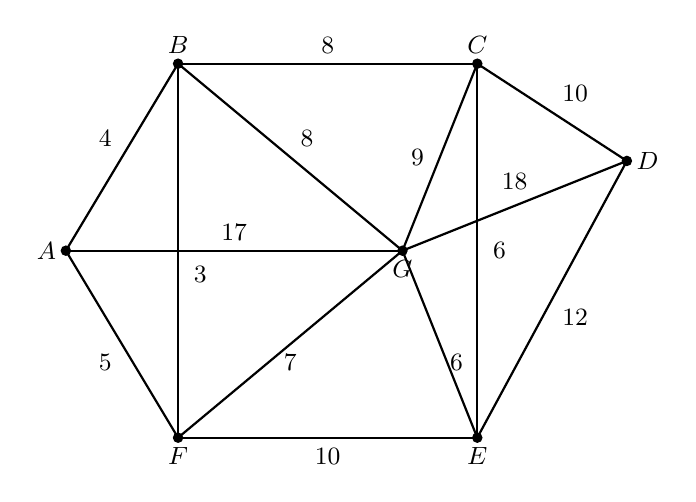
\begin{tikzpicture}[line cap=round, line join=round, >=stealth, scale=0.95]
			
			% Define vertices coordinates according to the graph structure
			\coordinate (A) at (-3.5, 0.0);
			\coordinate (B) at (-2.0, 2.5);
			\coordinate (C) at (2.0, 2.5);
			\coordinate (D) at (4.0, 1.2);
			\coordinate (E) at (2.0, -2.5);
			\coordinate (F) at (-2.0, -2.5);
			\coordinate (G) at (1.0, 0.0);
			
			% Draw edges
			% Outer boundary edges
			\draw[thick] (A) -- (B) node[midway, above left, font=\small] {$4$};
			\draw[thick] (B) -- (C) node[midway, above, font=\small] {$8$};
			\draw[thick] (C) -- (D) node[midway, above right, font=\small] {$10$};
			\draw[thick] (D) -- (E) node[midway, below right, font=\small] {$12$};
			\draw[thick] (E) -- (F) node[midway, below, font=\small] {$10$};
			\draw[thick] (F) -- (A) node[midway, below left, font=\small] {$5$};
			
			% Internal edges
			\draw[thick] (B) -- (F) node[midway, below right=2pt, font=\small] {$3$};
			\draw[thick] (C) -- (E) node[midway, right=2pt, font=\small] {$6$};
			\draw[thick] (A) -- (G) node[midway, above, font=\small] {$17$};
			\draw[thick] (B) -- (G) node[midway, above right, font=\small] {$8$};
			\draw[thick] (C) -- (G) node[midway, left=2pt, font=\small] {$9$};
			\draw[thick] (D) -- (G) node[midway, above=2pt, font=\small] {$18$};
			\draw[thick] (E) -- (G) node[midway, below right, font=\small] {$6$};
			\draw[thick] (F) -- (G) node[midway, below, font=\small] {$7$};
			
			% Plot vertex points
			\foreach \p in {A, B, C, D, E, F, G} {
				\fill (\p) circle (2.0pt);
			}
			
			% Vertex labels
			\node[left, font=\small] at (A) {$A$};
			\node[above, font=\small] at (B) {$B$};
			\node[above, font=\small] at (C) {$C$};
			\node[right, font=\small] at (D) {$D$};
			\node[below, font=\small] at (E) {$E$};
			\node[below, font=\small] at (F) {$F$};
			\node[below, font=\small] at (G) {$G$};
			
		\end{tikzpicture}
	\end{center}
	\begin{traloi}
		\dapan{145}
		
		Đây là bài toán người đưa thư: bác Shipper phải đi qua tất cả các cạnh và cuối cùng quay lại \(A\).
		
		Tổng thời gian đi qua mỗi con đường đúng một lần là
		\(4+8+10+12+10+5+3+6+17+8+9+18+6+7=123\) phút.
		
		Các đỉnh \(B,C,E,F,G\) có bậc chẵn, còn \(A,D\) có bậc lẻ. Muốn có một chu trình xuất phát và kết thúc tại \(A\), cần đi lặp thêm một đường ngắn nhất nối hai đỉnh bậc lẻ \(A,D\).
		
		Đường ngắn nhất là \(A\to B\to C\to D\), có thời gian \(4+8+10=22\) phút.
		
		Vậy thời gian ngắn nhất là \(123+22=145\) phút.
	\end{traloi}
\end{baitap}

\begin{baitap}
	%\textbf{Câu 3.}
	Trong không gian $Oxyz$, cho tam giác $ABC$ có $A(-4; -1; 2)$, $B(3; 5; -6)$ và $C(a; b; c)$. Biết trung điểm cạnh $AC$ thuộc trục tung, trung điểm cạnh $BC$ thuộc mặt phẳng $(Oxz)$. Tính $T = 2a + b - c$.
	\begin{traloi}
		\dapan{5}
		Gọi $M$ là trung điểm $AC \Rightarrow M\left(\frac{a-4}{2}; \frac{b-1}{2}; \frac{c+2}{2}\right)$.
		Vì $M \in Oy \Rightarrow \begin{cases} \frac{a-4}{2} = 0 \\ \frac{c+2}{2} = 0 \end{cases} \Rightarrow \begin{cases} a = 4 \\ c = -2 \end{cases}$.
		Gọi $N$ là trung điểm $BC \Rightarrow N\left(\frac{a+3}{2}; \frac{b+5}{2}; \frac{c-6}{2}\right)$.
		Vì $N \in (Oxz) \Rightarrow \frac{b+5}{2} = 0 \Rightarrow b = -5$.
		Do đó $C(4; -5; -2)$.
		Vậy $T = 2a + b - c = 2(4) + (-5) - (-2) = 8 - 5 + 2 = 5$.
	\end{traloi}
\end{baitap}
\begin{baitap}
	%\textbf{Câu 4.}
	Cho tập hợp $X = \{1; 2; 3; 4; 5; 6; 7; 8\}$. Gọi $S$ là tập hợp tất cả các số tự nhiên có 4 chữ số được lập từ các chữ số thuộc tập $X$. Chọn ngẫu nhiên một số từ tập hợp $S$. Xác suất để chọn được một số chia hết cho 3 bằng $\frac{a}{b}$ (với $a, b \in \mathbb{N}^*$, $\frac{a}{b}$ là phân số tối giản). Tính $T = a + b$.
	\begin{traloi}
		\dapan{2731}
		Trong $X$ có $2$ số chia hết cho $3$, $3$ số chia $3$ dư $1$ và $3$ số chia $3$ dư $2$.
		
		Gọi số cần tìm có dạng $ \overline{abcd} $. Đầu tiên, ta xem có bao nhiêu cách lập được $ \overline{abc} $ mà có tổng chia hết cho $ 3 $. Để tổng của ba chữ số này chia hết cho \(3\), bộ ba số dư có thể thuộc một trong bốn dạng:
		
		\[
		(0,0,0),\quad (1,1,1),\quad (2,2,2),\quad (0,1,2).
		\]
		
		Ba dạng đầu có lần lượt \(2^3,3^3,3^3\) cách. Riêng dạng thứ tư \((0,1,2)\):
		\begin{itemize}
			\item chọn một chữ số dư \(0\): \(2\) cách;
			\item chọn một chữ số dư \(1\): \(3\) cách;
			\item chọn một chữ số dư \(2\): \(3\) cách;
			\item ba chữ số này (khác nhau) mà có thể nằm ở ba vị trí \(a,b,c\) nên có \(3!=6\) cách.
		\end{itemize}			
		Do đó dạng thứ tư có \(6\cdot2\cdot3\cdot3=108\) cách. Vì vậy tổng cách lập được $ \overline{abc} $ mà có tổng chia hết cho $ 3 $ là:
		\[
		2^3+3^3+3^3+6\cdot2\cdot3\cdot3
		=8+27+27+108
		=170.
		\]
		
		Do tính đối xứng, hai trường hợp tổng chia $3$ dư $1$ và dư $2$ đều có
		$\frac{8^3-170}{2}=171$ cách. Sau khi có được $ \overline{abc} $, ta cần xem có bao nhiêu cách lập $ d $. 
		\begin{itemize}
			\item nếu \(a+b+c\equiv0\), thì chọn \(d\) chia hết cho $ 0 $: có \(2\) cách;
			\item nếu \(a+b+c\equiv1\), thì chọn \(d\) chia hết cho $ 2 $: có \(3\) cách;
			\item nếu \(a+b+c\equiv2\), thì chọn \(d\) chia hết cho $ 1 $: có \(3\) cách.
		\end{itemize}
		Do đó số trường hợp thuận lợi là
		$$170\cdot2+171\cdot3+171\cdot3=1366.$$
		
		Suy ra $P=\frac{1366}{8^4}=\frac{683}{2048}$, nên $T=683+2048=2731$.
	\end{traloi}
\end{baitap}

\begin{baitap}
	%\textbf{Câu 5.}
	Một quần thể vi khuẩn được nuôi cấy trong phòng thí nghiệm. Nồng độ dinh dưỡng $S$ (đơn vị: $\mathrm{mg/\ell}$) thay đổi theo thời gian $t$ giờ ($t \ge 0$) được mô hình hóa bởi hàm số: $S(t) = \frac{10t + 5}{t + 1}$. Biết tốc độ sinh trưởng $V$ của vi khuẩn phụ thuộc vào nồng độ dinh dưỡng theo hàm số $V(S) = \frac{5S}{S + 2}$. Khi thời gian $t$ kéo dài, tốc độ sinh trưởng $V$ tăng dần và ổn định quanh một ngưỡng $K$ nhất định. Hỏi sau bao nhiêu phút thì tốc độ sinh trưởng của vi khuẩn đạt $90\%$ ngưỡng $K$?
	\begin{traloi}
		\dapan{15}
		Ta có $\lim\limits_{t\to+\infty}S(t)=10$, nên
		$$K=V(10)=\frac{25}{6}.$$
		
		Khi $V(S)=90\%K=\frac{15}{4}$, ta có
		$$\frac{5S}{S+2}=\frac{15}{4}\Rightarrow S=6.$$		
		Do đó $\frac{10t+5}{t+1}=6\Rightarrow t=\frac14$ giờ $=\qty{15}{\minute}$.
	\end{traloi}
\end{baitap}

\begin{baitap}
	%\textbf{Câu 6.}
	Trong không gian với hệ trục tọa độ $Oxyz$, mặt phẳng $(P) : bcx + acy + abz - abc = 0$ qua điểm $M(2; 4; 8)$ và cắt các tia $Ox, Oy, Oz$ lần lượt tại $A, B, C$ sao cho $OA = 2OB = 4OC$. Tính $T = a + b + c$.
	\begin{traloi}
		\dapan{73,5}
		Ta viết lại phương trình của mặt phẳng \((P)\): $$(P):\frac{x}{a}+\frac{y}{b}+\frac{z}{c}=1,$$ với $a,b,c>0$.
		
		Từ $OA=2OB=4OC$ suy ra $a=2b=4c$, nên $a=4c,\ b=2c$.	Mà $M(2;4;8)\in(P)$ nên
		\[
		\frac{2}{4c}+\frac{4}{2c}+\frac{8}{c}=1
		\Rightarrow c=\frac{21}{2}.
		\]
		Suy ra $a=42,\ b=21,\ c=10{,}5$. Vậy $T=a+b+c=73{,}5$.
	\end{traloi}
\end{baitap}
